\documentclass{article}

\makeatletter
\renewcommand{\fnum@figure}{Εικόνα \thefigure}
\makeatother

\usepackage[greek, english]{babel}
\usepackage{alphabeta}
\usepackage{atbegshi, picture}

% Set page size and margins
% Replace `letterpaper' with`a4paper' for UK/EU standard size
\usepackage[letterpaper,top=2cm,bottom=2cm,left=3cm,right=3cm,marginparwidth=1.75cm]{geometry}

% Useful packages
\usepackage{amsmath}
\usepackage{graphicx}
\usepackage[colorlinks=true, allcolors=blue]{hyperref}
\usepackage[utf8]{inputenc}
\usepackage{indentfirst}

\newcommand\T{\rule{0pt}{2.6ex}}       % Top strut
\newcommand\B{\rule[-1.2ex]{0pt}{0pt}} 


\addto\captionsenglish{
  \renewcommand{\contentsname}
    {Περιεχόμενα}
}

% \title{Feasibility Study}
% \date{}

\begin{document}
% \maketitle

\begin{titlepage}
   \begin{center}
       \vspace*{1cm}

       \textbf{\huge Use Cases}

       \vspace{0.5cm}
        Τεχνολογία Λογισμικού
            
       \vspace{1cm}

       \textbf{Αγγελική Κούρου\\Κατερίνα Μητροπούλου}
       
       \begin{figure}[!htb]
        \centering
        
\includegraphics[width=0.5\textwidth]{logo.png}
        \end{figure}
        
        \vspace{0.5cm}
        
        \begin{figure}[!htb]
        \centering
        \includegraphics[width=0.5\textwidth]{UoP.jpg}
        \end{figure}


       \vfill
            
       Τεχνικό Κείμενο για την Τεχνολογία Λογισμικού\\
            
       \vspace{0.5cm}
            
       CEID, ECE\\
       University of Patras\\
            
   \end{center}
\end{titlepage}



\noindent Η ομάδα μας

\begin{enumerate}
  \item Βεργίνης Δημήτριος, ΑΜ: 1066634 , ECE
  \item Βλαχογιάννης Δημήτριος, ΑΜ: 1067371, CEID
  \item Κούρου Αγγελική, ΑΜ: 1067499 , CEID
  \item Μητροπούλου Αικατερίνα - Quality Manager, ΑΜ: 1067409, CEID
  \item Στεφανίδης Μάριος - Project Manager, ΑΜ:1067458, CEID
\end{enumerate}

{
  \hypersetup{linkcolor=black}
  \tableofcontents
}

\section{Εισαγωγή}

Τα Use Cases αποτελούν ένα σύνολο δραστηριοτήτων ή βημάτων που λαμβάνουν χώρα κατά την πλοήγηση ενός χρήστη (ή ρόλου, γνωστού στην UML ως ηθοποιού) σε ένα σύστημα, για να επιτευχθεί ένας στόχος. Ο ηθοποιός μπορεί να είναι άνθρωπος ή κάποιο άλλο εξωτερικό σύστημα. 
Για την ανάπτυξη ενός use case χρησιμοποιούνται τα διαγράμματα περιπτώσεων χρήσης, καθώς και λεκτική περιγραφή των περιπτώσεων αυτών.

\section{Διάγραμμα Περιπτώσεων Χρήσης}

Παρακάτω παρουσιάζεται το διάγραμμα περιπτώσεων χρήσης. Για την καλύτερη κατανόηση του διαγράμματος σημειώνεται ότι:

\begin{enumerate}
  \item Τα σκίτσα με τους ανθρώπους αντιστοιχούν στους ηθοποιούς του εκάστοτε use case, δηλαδή τους εμπλεκόμενους
  \item Οι μπλε ελλείψεις αντιστοιχούν στα use cases
  \item Οι μαύρες γραμμές απεικονίζουν άμεση συσχέτιση μεταξύ ενός ηθοποιού και μίας περίπτωσης χρήσης
  \item Οι μαύρες διακεκομμένες γραμμές απεικονίζουν τη σχέση εξάρτησης μεταξύ δύο περιπτώσεων χρήσης, δηλαδή το use case στο οποίο δείχνει το βέλος δεν μπορεί να υπάρξει αν δεν έχει προηγηθεί το use case από το οποίο ξεκινάει το βέλος  
\end{enumerate}


\newpage

\begin{figure}[!htb]
        \centering
        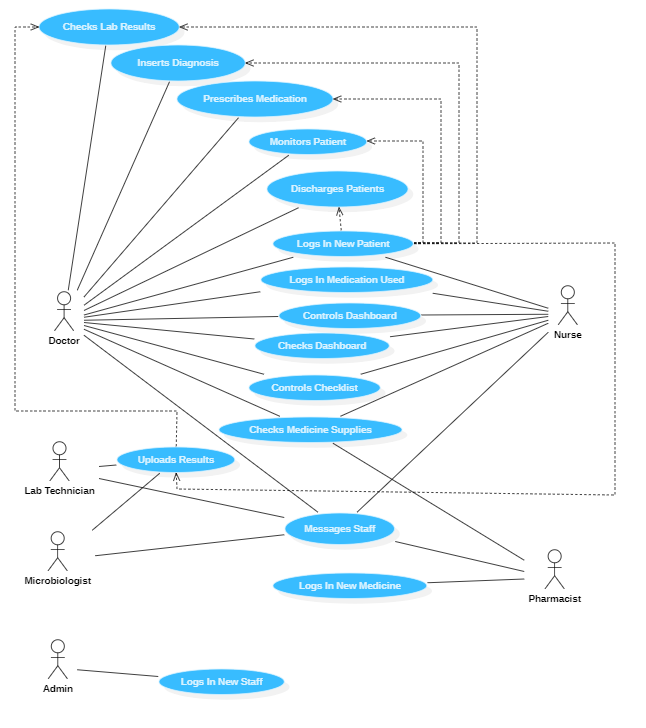
\includegraphics[width=1.0\textwidth]{UML.png}
        \end{figure}
        
        \vspace{0.5cm}

\section{Use Case 1: Διάγνωση Ασθενούς}

Παρακάτω θα αναλυθεί το σενάριο χρήσης του \textbf{Medic World} κατά το οποίο ένας γιατρός καταχωρεί την διάγνωση στην καρτέλα ενός ασθενούς.

\subsection{Περιγραφή}

\begin{center}
     \begin{tabular}{|l|l|}
     \hline
      \textbf{Περίπτωση Χρήσης 1} & Ο γιατρός εισάγει τη διάγνωση ενός ασθενούς \T\B \\ 
      \hline
      \textbf{Ηθοποιός} & Γιατρός \T\B \\
      \hline
      \textbf{Σενάριο Περίπτωσης Χρήσης} & Ένας από τους ασθενής χρείαζεται διάγνωση, οπότε \T\\& ο γιατρός εισέρχεται στην καρτέλα του, μελετάει τα\\& αποτελέσματα των εξετάσεών του και καταλήγει σε διάγνωση \B \\
      \hline
      \textbf{Αφορμή} & Ασθενής χρειάζεται διάγνωση \T\B \\
      \hline
      \textbf{Προαπαιτούμενο 1} & Να έχει καταχωρηθεί ο ασθενής στο σύστημα \T\B \\
      \hline
      \textbf{Προαπαιτούμενο 2} & Να είναι έτοιμα τα αποτελέσματα των εργαστηριακών εξετάσεων \T\B \\
      \hline
     \end{tabular}
 \end{center}
 
 \subsection{Αναλυτικό Σενάριο Χρήσης}
 
 \begin{center}
     \begin{tabular}{|l|l|}
     \hline
      \textbf{Περιγραφή} & Αυτό το σενάριο περιγράφει μια κατάσταση όπου χρειάζεται \T \\& η πλοήγηση σε τέσσερις καρτέλες, οι οποίες τελικά\\& οδηγούν στην επίτευξη του στόχου. \B \\ 
      \hline
      \textbf{Βήμα 1} & Ο γιατρός από το κεντρικό μενού επιλέγει το εικονίδιο \T \\& "Patients" \B \\
      \hline
      \textbf{Βήμα 2} & Ο γιατρός επιλέγει τον ασθενή που χρειάζεται διάγνωση \T\B \\
      \hline
      \textbf{Βήμα 3} & Ο γιατρός εξετάζει την κατάσταση του ασθενούς \T\B \\
      \hline
      \textbf{Βήμα 4} & Ο γιατρός εξετάζει το ιστορικό του ασθενούς \T\B \\
      \hline
      \textbf{Βήμα 5} & Ο γιατρός επιλέγει τα "lab results" \T\B \\
      \hline
      \textbf{Βήμα 6} & Ο γιατρός μελετάει τα "lab results" \T\B \\
      \hline
      \textbf{Βήμα 7} & Ο γιατρός επιλέγει το πλήκτρο "Diagnosis" \T\B \\
      \hline
      \textbf{Βήμα 8} & Ο γιατρός εισάγει τη νέα διάγνωση \T\B \\
      \hline
      \textbf{Βήμα 9} & Ο γιατρός επιλέγει το πλήκτρο ολοκλήρωσης \T\B \\
      \hline
      \textbf{Βήμα 10} & Στην καρτέλα του ασθενούς εμφανίζεται η διάγνωση \T\B \\
      \hline
     \end{tabular}
 \end{center}
 

 
 \section{Use Case 2: Απασχόληση Χειρουργείου}
 
 Παρακάτω θα αναλυθεί το σενάριο χρήσης του \textbf{Medic World} κατά το οποίο ένας χρήστης επιθυμεί να δηλώσει στο σύστημα τη χρήση ενός χειρουργείου.

\subsection{Περιγραφή}

\begin{center}
     \begin{tabular}{|l|l|}
     \hline
      \textbf{Περίπτωση Χρήσης 2} & Ο χρήστης δηλώνει την απασχόληση χειρουργείου \T\B \\ 
      \hline
      \textbf{Ηθοποιός} & Γιατρός \T\B \\
      \hline
      \textbf{Σενάριο Περίπτωσης Χρήσης} & Ένας γιατρός πρόκειται να εισάγει έναν ασθενή \T \\& σε κάποιο χειρουργείο και χρειάζεται να καταχωρηθεί\\& στην καρτέλα των χειρουργείων, ότι το συγκεκριμένο\\& δωμάτιο δε θα είναι διαθέσιμο για κάποιο χρονικό διάστημα \B \\
      \hline
      \textbf{Ηθοποιοί} & Γιατρός, Νοσηλευτής \T\B \\
      \hline
      \textbf{Αφορμή} & Ασθενής χρειάζεται χειρουργείο \T\B \\
      \hline
      \textbf{Προαπαιτούμενο 1} & Να έχει καταχωρηθεί ο ασθενής \T\B \\
      \hline
      \textbf{Πρoαπαιτούμενο 2} & Να έχει πραγματοποιηθεί διάγνωση του ασθενούς \T\B \\
      \hline
      \textbf{Προαπαιτούμενο 3} & Η διάγνωση να απαιτεί την εισαγωγή σε χειρουργείο \T\B \\
      \hline
     \end{tabular}
 \end{center}
 
 \subsection{Αναλυτικό Σενάριο Χρήσης}
 
 \begin{center}
     \begin{tabular}{|l|l|}
     \hline
      \textbf{Περιγραφή} & Αυτό το σενάριο περιγράφει μια κατάσταση όπου χρείαζεται \T \\& η πλοήγηση σε τέσσερις καρτέλες, οι οποίες\\& οδηγούν στην επίτευξη του στόχου. \B \\ 
      \hline
      \textbf{Βήμα 1} & Ο χρήστης επιλέγει από το κεντρικό μενού το εικονίδιο \T \\& "Checklist" \B \\
      \hline
      \textbf{Βήμα 2} & Ο χρήστης επιλέγει από το μενού του Checklist \T \\& τα "Operating Rooms" \B \\
      \hline
      \textbf{Βήμα 3} & Ο χρήστης ελέγχει τη διαθεσιμότητα των χειρουργείων \T\B \\
      \hline
      \textbf{Βήμα 4} & Ο χρήστης επιλέγει ένα από τα διαθέσιμα χειρουργεία \T\B \\
      \hline
      \textbf{Βήμα 5} & Ο χρήστης οδηγείται σε μία φόρμα συμπλήρωσης στοιχείων \T\B \\
      \hline
      \textbf{Βήμα 6} & Ο χρήστης εισάγει τα στοιχεία που απαιτεί η φόρμα\T\B \\
      \hline
      \textbf{Βήμα 7} & Ο χρήστης μέσω του πλήκτρου "Done" επιλέγει την \T \\& ολοκλήρωση της διαδικασίας \B \\
      \hline
      \textbf{Βήμα 8} & Στην καρτέλα διαθεσιμότητας των χειρουργείων \T \\& εμφανίζεται πλέον ως μη διαθέσιμο το χειρουργείο\\& που επέλεξε νωρίτερα ο χρήστης \B \\
      \hline
     \end{tabular}
 \end{center}
 

  \section{Use Case 3: Καταχώρηση Νέου Φαρμάκου }
 
 Παρακάτω θα αναλυθεί το σενάριο χρήσης του \textbf{Medic World} κατά το οποίο ένας φαρμακοποιός επιθυμεί να εισάγει στο σύστημα ένα νέο φάρμακο.
 
\subsection{Περιγραφή}

\begin{center}
     \begin{tabular}{|l|l|}
     \hline
      \textbf{Περίπτωση Χρήσης 3} & Ο χρήστης εισάγει νέο φάρμακο στην καρτέλα προμηθειών \T\B \\ 
      \hline
      \textbf{Ηθοποιός} & Φαρμακοποιός \T\B \\
      \hline
      \textbf{Σενάριο Περίπτωσης Χρήσης} & Από το νοσοκομείο έγινε αγορά ενός νέου φαρμάκου \T \\& και ο φαρμακοποιός καλείται να το καταχωρήσει \\& στην καρτέλα προμηθειών \B \\
      \hline
      \textbf{Αφορμή} & Η αγορά νέου φαρμάκου \T\B \\
      \hline
      \textbf{Προαπαιτούμενο 1} &  Να μην υπάρχει ήδη το φάρμακο στην καρτέλα προμηθειών \T\B \\
      \hline
     \end{tabular}
 \end{center}
 
 \subsection{Αναλυτικό Σενάριο Χρήσης}
 
 \begin{center}
     \begin{tabular}{|l|l|}
     \hline
      \textbf{Περιγραφή} & Αυτό το σενάριο περιγράφει μια κατάσταση όπου χρειάζεται \T \\& πλοήγηση σε δύο καρτέλες. οι οποίες οδηγούν στην επίτευξη \\& του στόχου  \B \\ 
      \hline
      \textbf{Βήμα 1} & Ο φαρμακοποιός επιλέγει από το κεντρικό μενού το εικονίδιο \T \\&  "Medicine Supplies" \B \\
      \hline
      \textbf{Βήμα 2} & Ο φαρμακοποιός επιλέγει το κουμπί "New Medicine" \T\B \\
      \hline
      \textbf{Βήμα 3} & Ο φαρμακοποιός συμπληρώνει τον τύπο του φαρμάκου \T \\& (λ.χ. αντιβιοτικό) \B \\
      \hline
      \textbf{Βήμα 4} & Ο φαρμακοποιός καταχωρεί το όνομα του φαρμάκου \T\B \\
      \hline
      \textbf{Βήμα 5} & Ο φαρμακοποιός συμπληρώνει τα τεμάχια που είναι σε απόθεμα \T\B \\
      \hline
      \textbf{Βήμα 6} & Ο φαρμακοποιός καταχωρεί τρία νούμερα για την περιγραφή \T \\&  της πληρότητας \B \\
      \hline
      \textbf{Βήμα 7} & Ο φαρμακοποιός επιλέγει το κουμπί "Done" \T\B \\
      \hline
      \textbf{Βήμα 8} & Στην καρτέλα διαθεσιμότητας φαρμάκων, επιλέγοντας \T \\ & την κατηγορία που αφορά το νεοεισαχθέν φάρμακο, \\& εμφανίζεται πλέον το νέο προϊόν \B \\
      \hline
     \end{tabular}
 \end{center}

\end{document}